\chapter{Описание структур}

\begin{lstlisting}[language=C]
struct audit_names;
struct filename {
	const char			*name;	/* pointer to actual string */
	const __user char	*uptr;	/* original userland pointer */
	int					refcnt;
	struct audit_names	*aname;
	const char			iname[];
};
static_assert(offsetof(struct filename, iname) % sizeof(long) == 0);
\end{lstlisting}

\begin{lstlisting}[language=C]
/* When fs/namei.c:getname() is called, we store the pointer in name and bump
 * the refcnt in the associated filename struct.
 *
 * Further, in fs/namei.c:path_lookup() we store the inode and device.
 */
struct audit_names {
	struct list_head		list;		/* audit_context->names_list */

	struct filename			*name;
	int						name_len;	/* number of chars to log */
	bool					hidden;		/* don't log this record */

	unsigned long			ino;
	dev_t					dev;
	umode_t					mode;
	kuid_t					uid;
	kgid_t					gid;
	dev_t					rdev;
	u32						osid;
	struct audit_cap_data	fcap;
	unsigned int			fcap_ver;
	unsigned char			type;		/* record type */
	/*
	* This was an allocated audit_names and not from the array of
	* names allocated in the task audit context.  Thus this name
	* should be freed on syscall exit.
	*/
	bool					should_free;
};   
\end{lstlisting}

\clearpage

\begin{lstlisting}[language=C]
struct open_flags {
	int 		open_flag;
	umode_t 	mode;
	int 		acc_mode;
	int 		intent;
	int 		lookup_flags;
};
\end{lstlisting}

\begin{lstlisting}[language=C]
#define EMBEDDED_LEVELS 2
struct nameidata {
	struct path		path;
	struct qstr		last;
	struct path		root;
	struct inode	*inode; /* path.dentry.d_inode */
	unsigned int	flags, state;
	unsigned		seq, m_seq, r_seq;
	int				last_type;
	unsigned		depth;
	int				total_link_count;
	struct saved {
		struct path link;
		struct delayed_call done;
		const char *name;
		unsigned seq;
	} *stack, internal[EMBEDDED_LEVELS];
	struct filename	*name;
	struct nameidata *saved;
	unsigned		root_seq;
	int				dfd;
	kuid_t			dir_uid;
	umode_t			dir_mode;
} __randomize_layout;
\end{lstlisting}

\chapter{Схема алгоритма функции open}

\begin{center}
	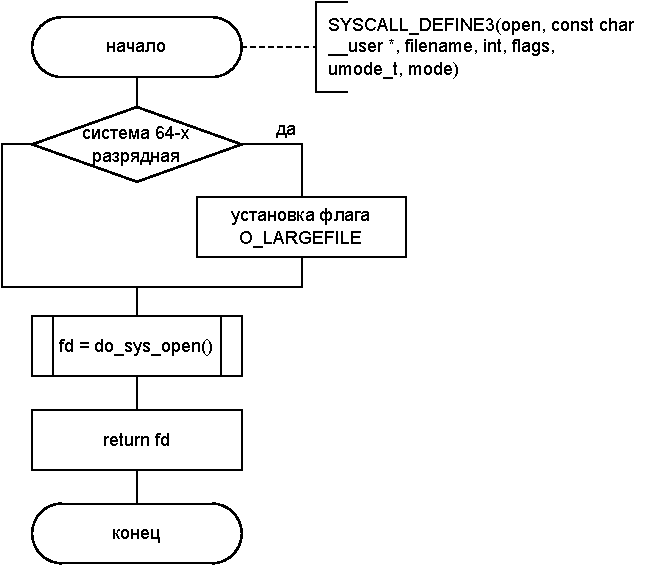
\includegraphics[]{open.pdf}
\end{center}

\begin{center}
	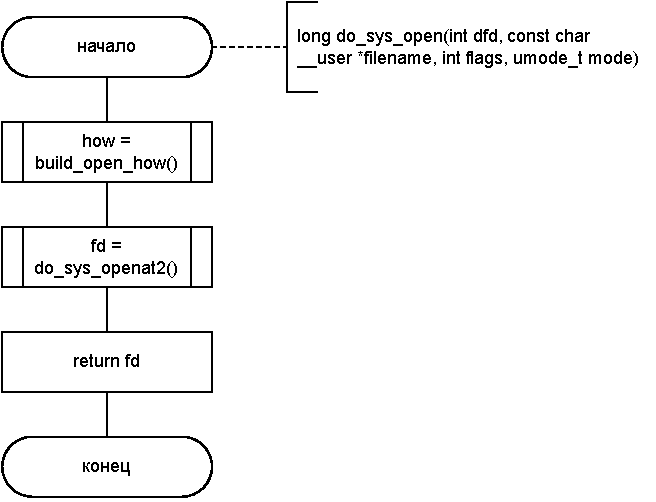
\includegraphics[]{do_sys_open.pdf}
\end{center}

\begin{center}
	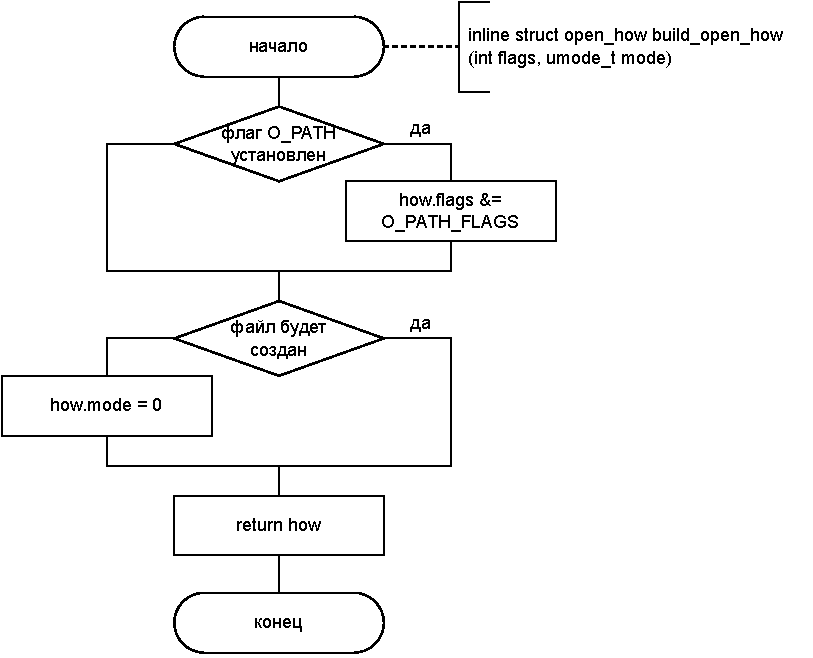
\includegraphics[]{build_open_how.pdf}
\end{center}

\begin{center}
	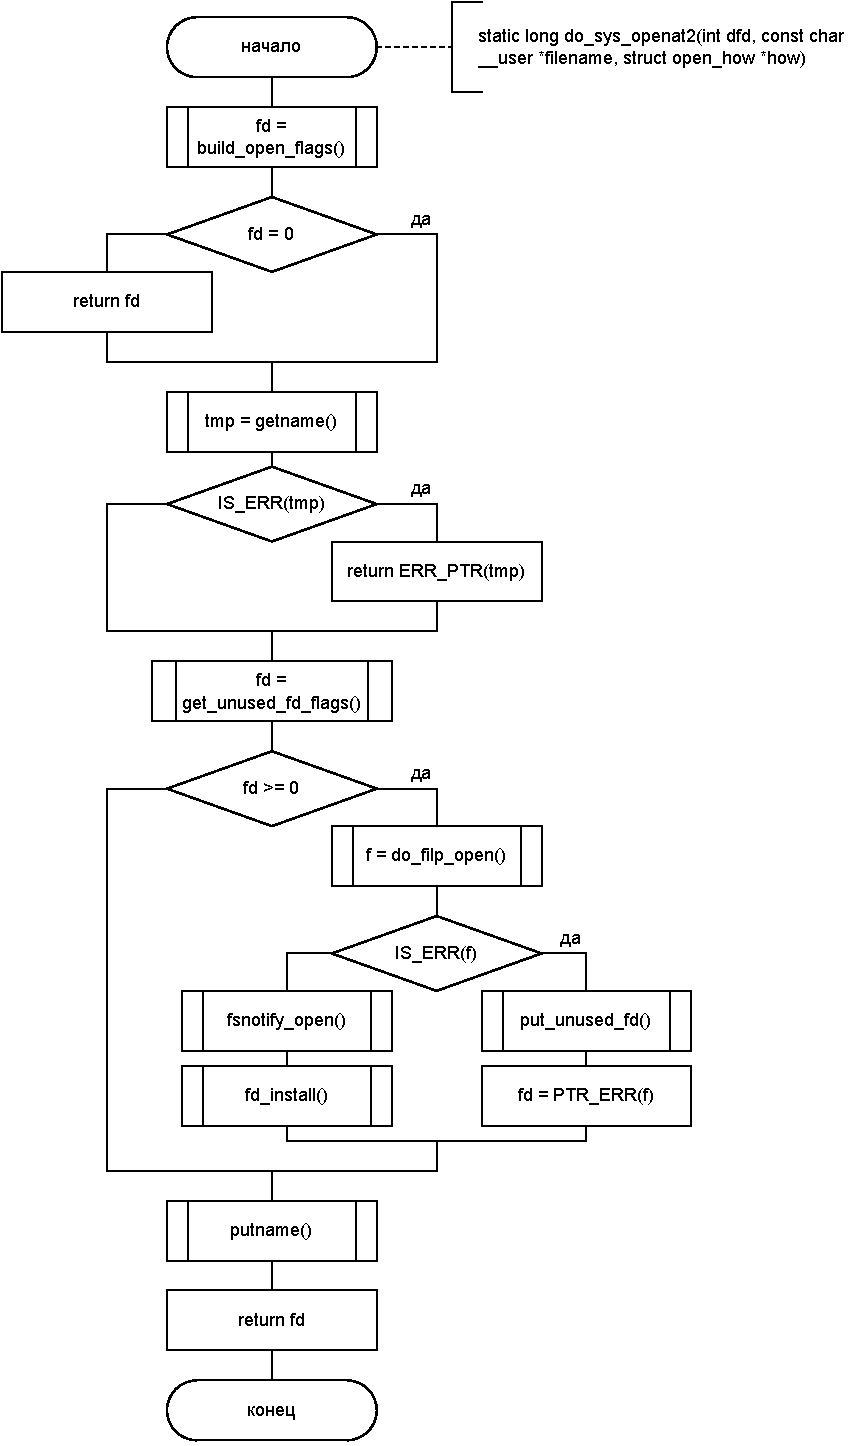
\includegraphics[]{do_sys_openat2.pdf}
\end{center}

\begin{center}
	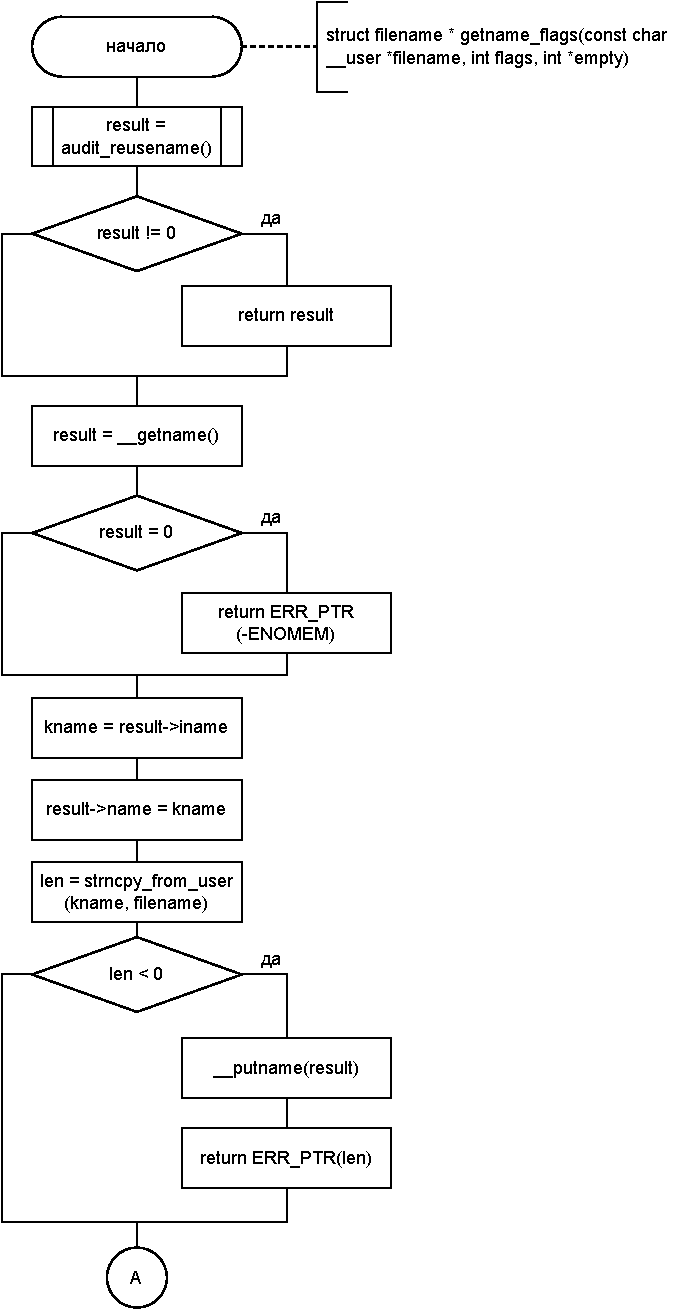
\includegraphics[]{getname-1.pdf}
\end{center}

\begin{center}
	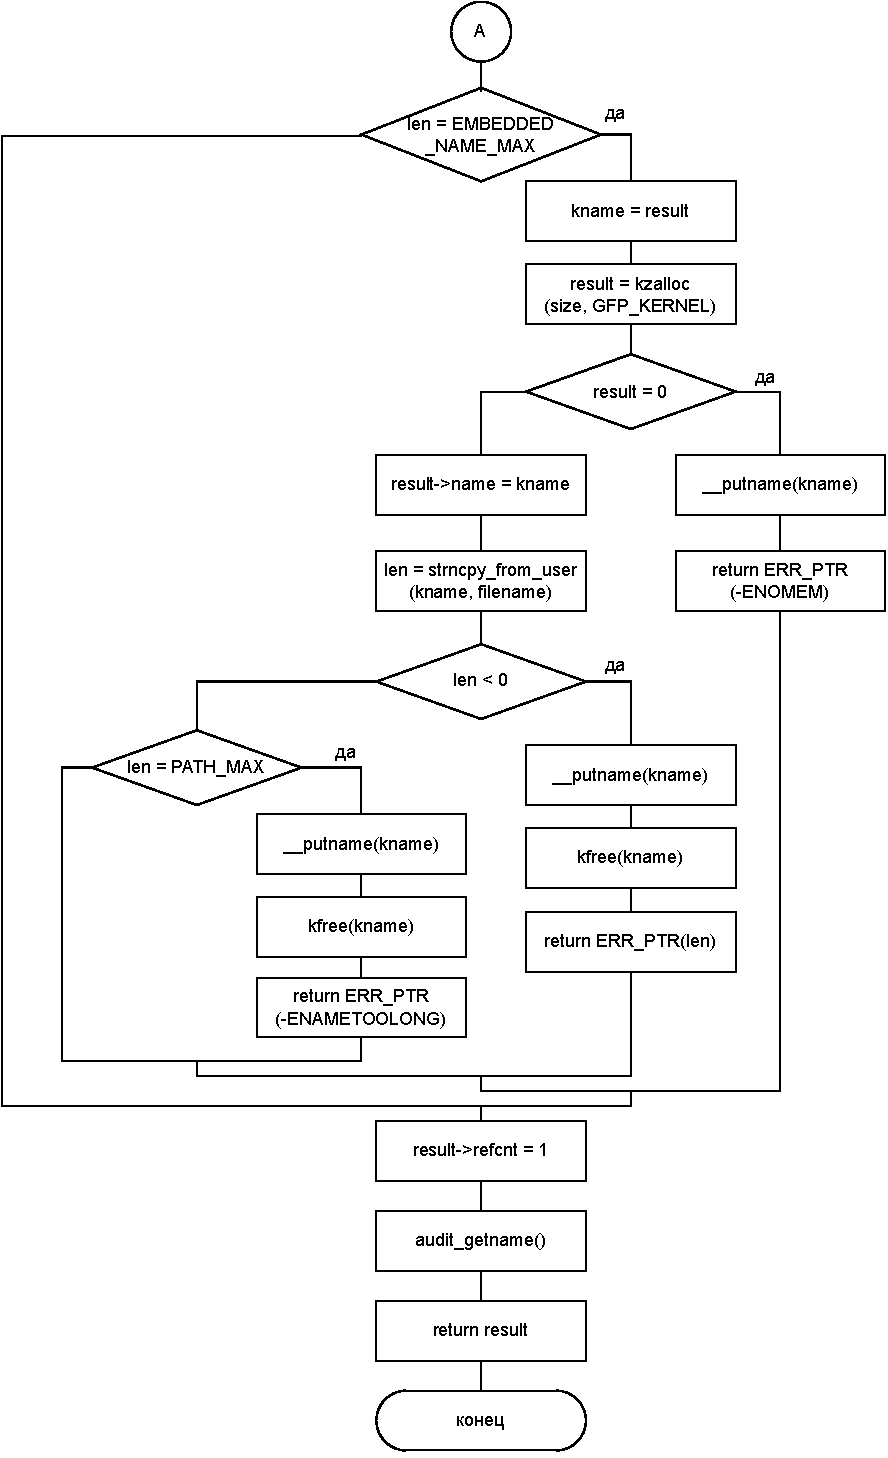
\includegraphics[]{getname-2.pdf}
\end{center}

\begin{center}
	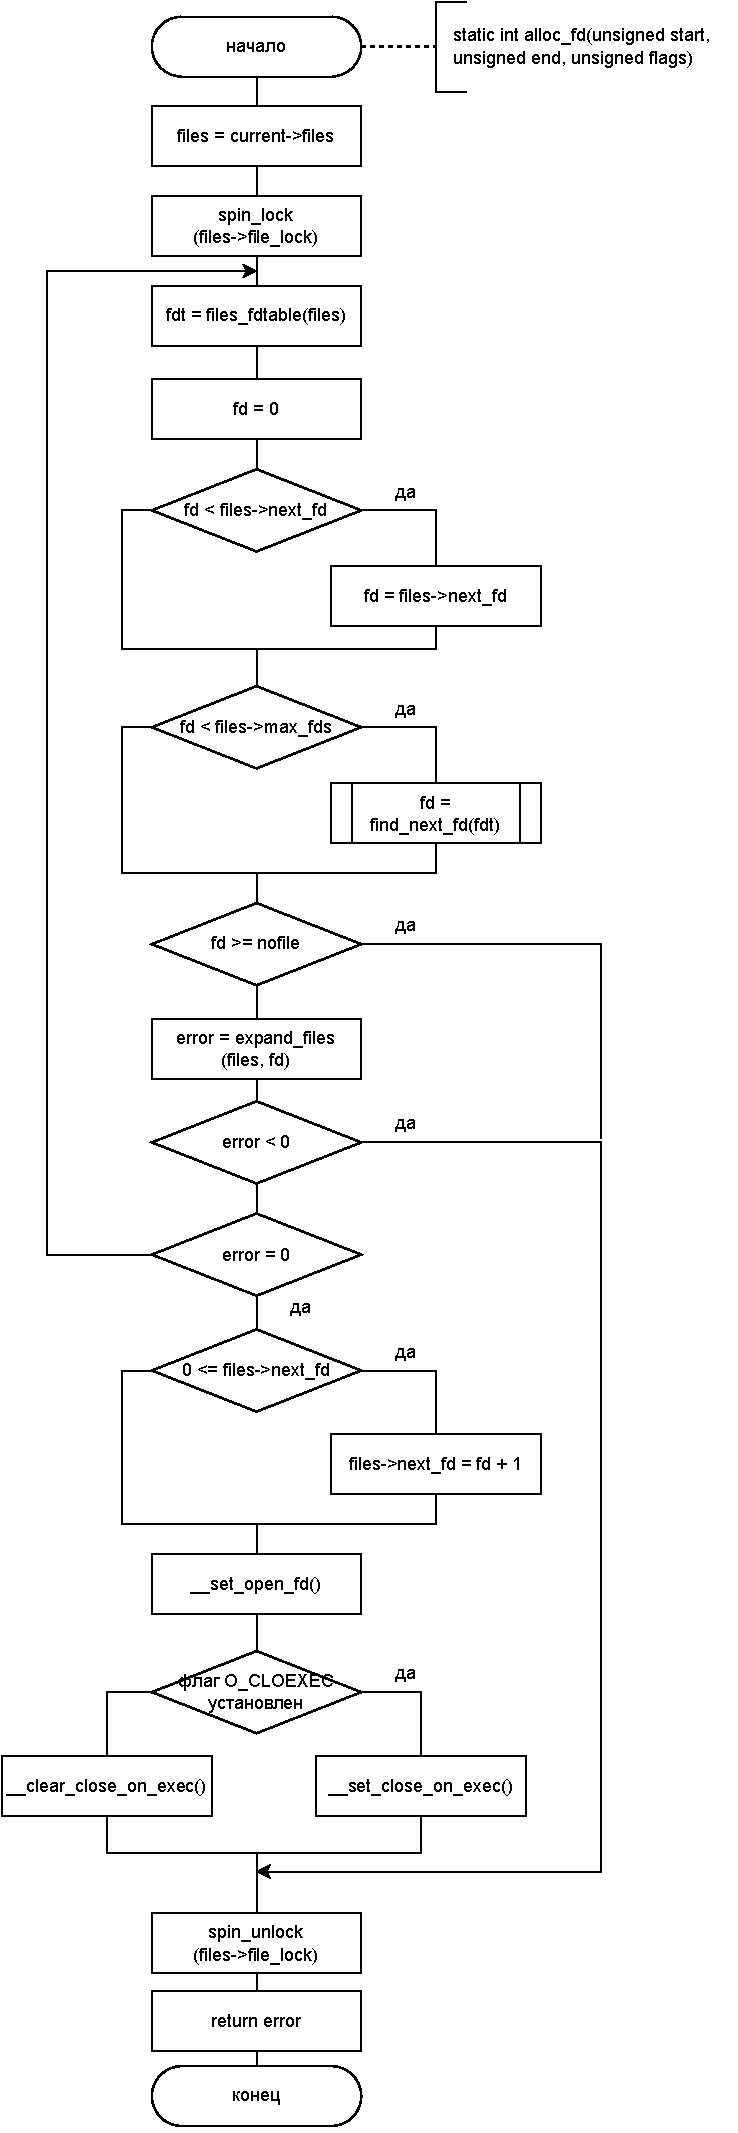
\includegraphics[height=\textheight]{get_unused_fd_flags.pdf}
\end{center}

\begin{center}
	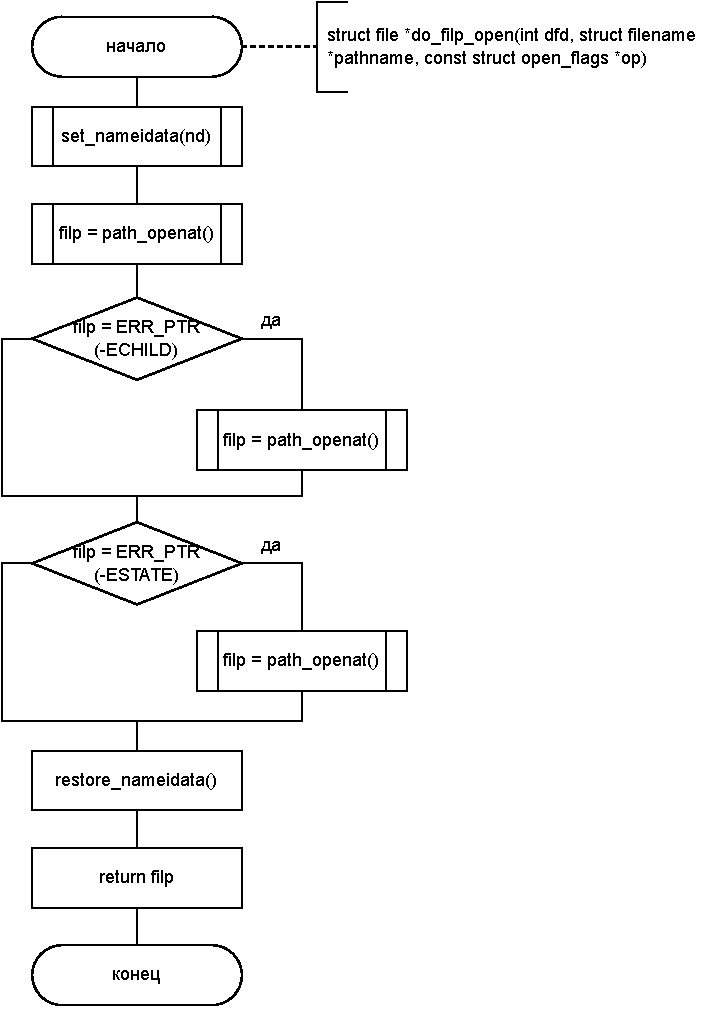
\includegraphics[]{do_filp_open.pdf}
\end{center}

\begin{center}
	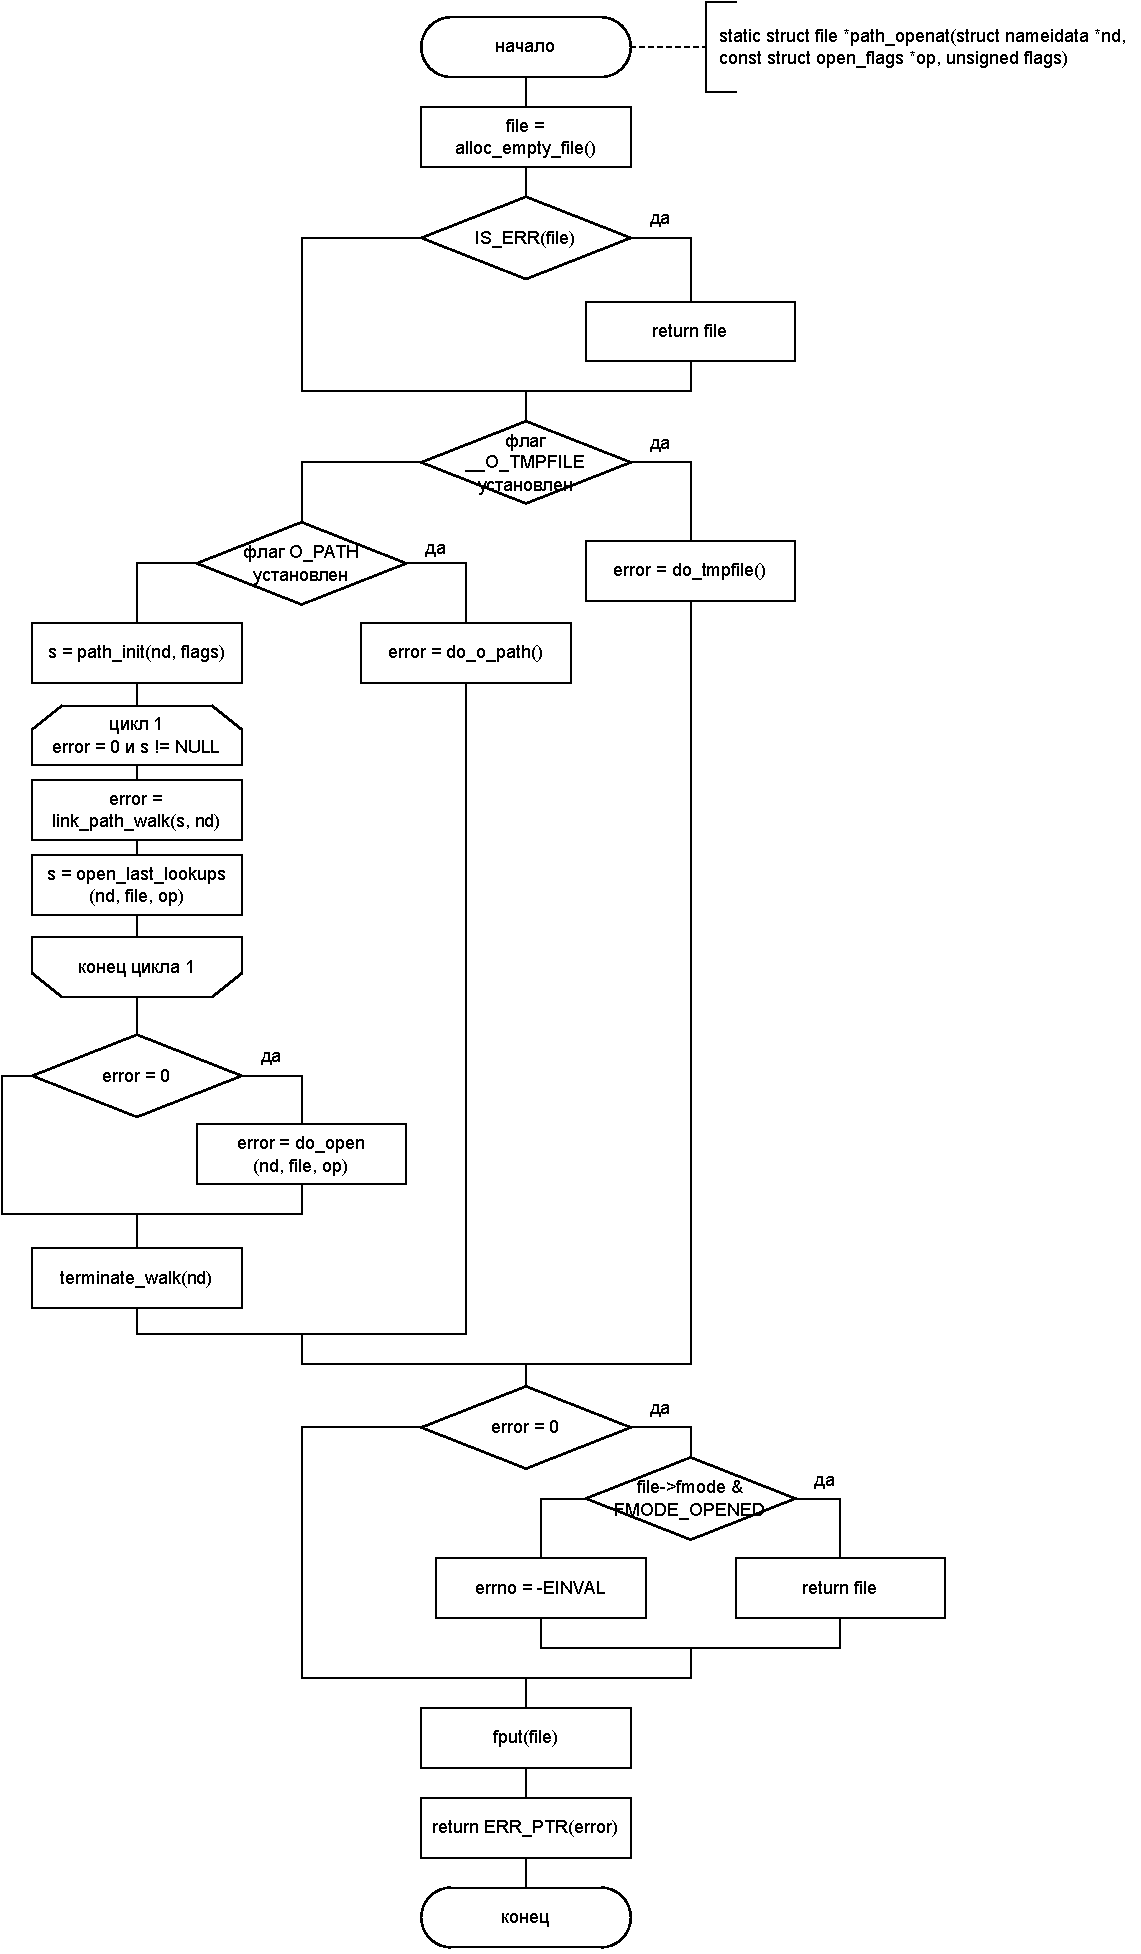
\includegraphics[height=\textheight]{path_openat.pdf}
\end{center}

\begin{center}
	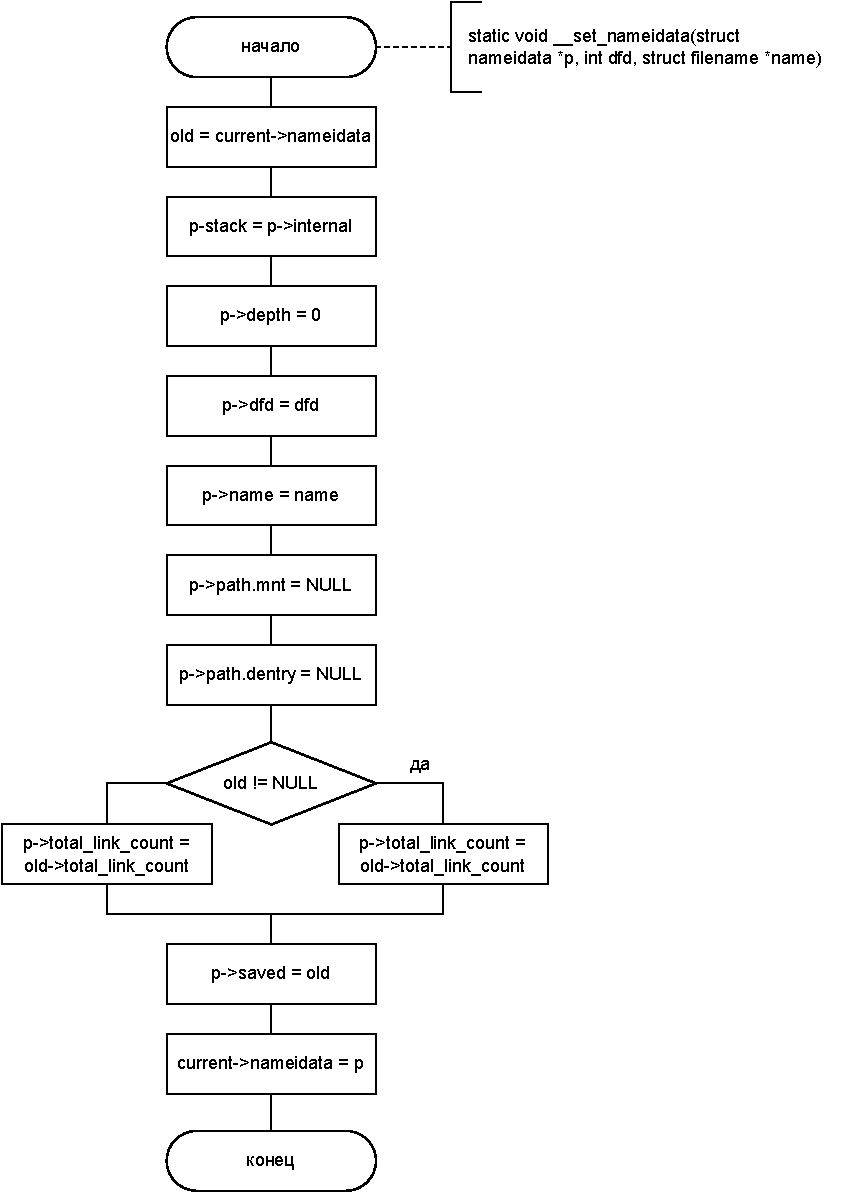
\includegraphics[]{set_nameidata.pdf}
\end{center}

\begin{center}
	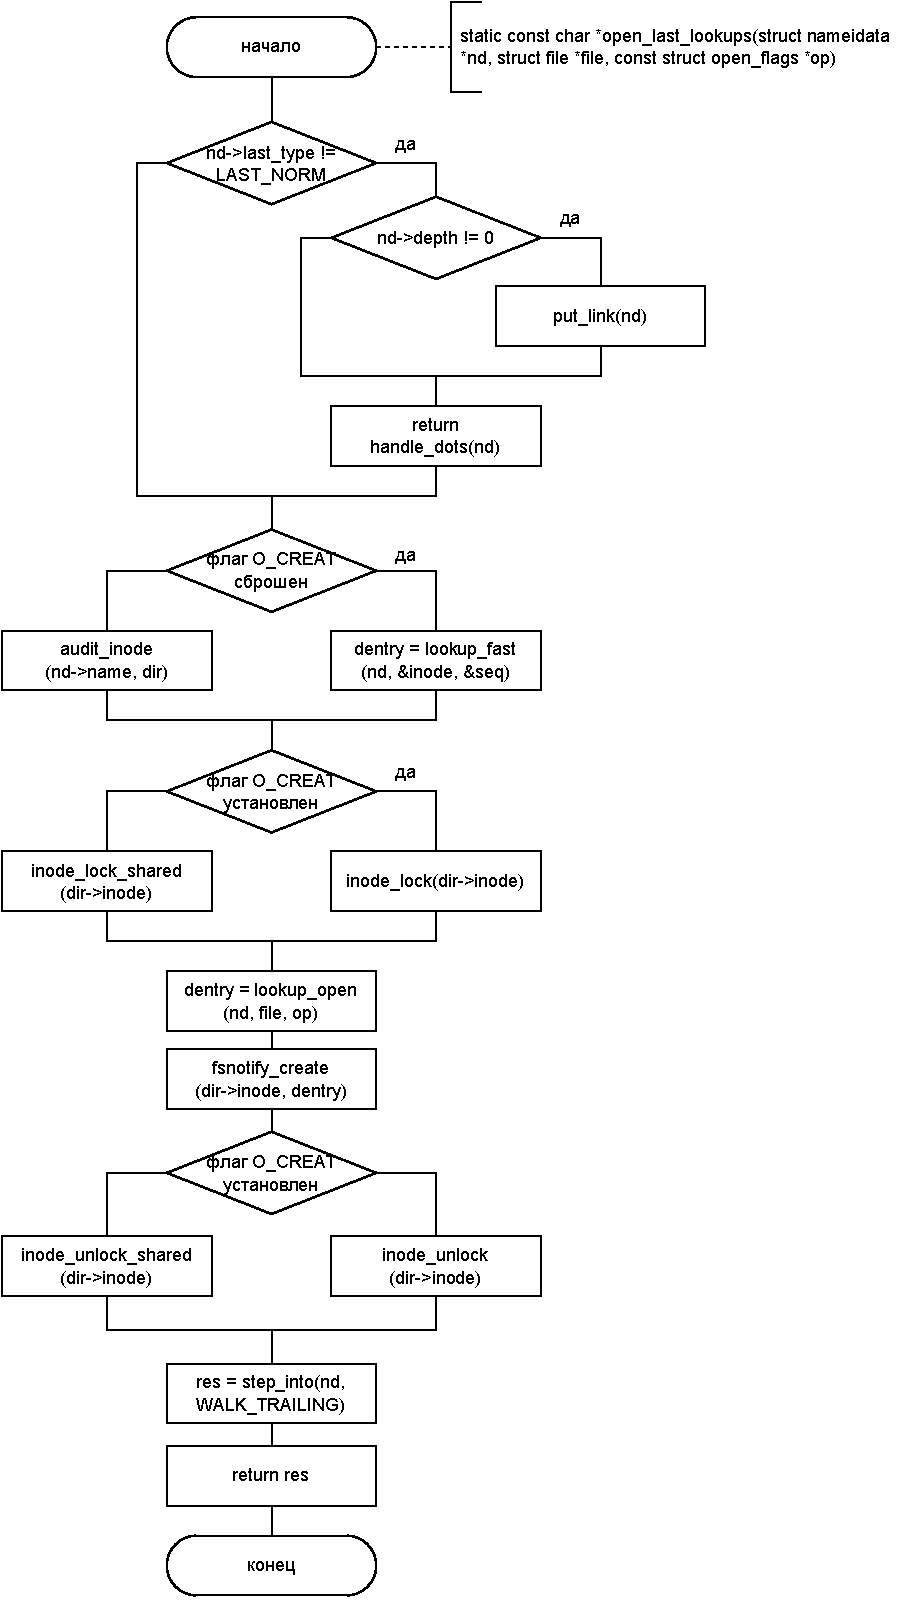
\includegraphics[height=\textheight]{open_last_lookups.pdf}
\end{center}
